Ce rapport présente les différents programmes réalisés dans le cadre du cours de traitement d'images. Ces programmes avaient pour but de segmenter des images IRM afin d'identifier la tumeur dans chaque image.\\

Deux images sont disponibles: une image avant le traitement du patient (figure \ref{irm1}) et une autre image correspondant à une IRM effectuée après que le patient ait commencé sont traitement (figure \ref{irm2}). En segmentant l'image, nous pouvons donc identifier la tumeur et calculer sa surface afin de comparer l'évolution de sa taille avant et après le traitement, et ainsi dire si le traitement a été efficace.\\

\begin{figure}[t!]
    \centering
    \begin{subfigure}[b]{0.5\textwidth}
        \centering
        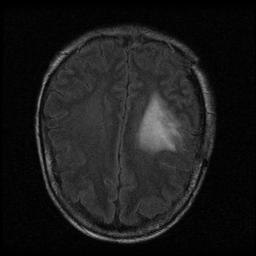
\includegraphics[width=0.95\textwidth]{images/IRMcoupe17-t1.jpg}
	\caption{IRM avant traitement}\label{irm1}
    \end{subfigure}%
    ~ 
    \begin{subfigure}[b]{0.5\textwidth}
        \centering
        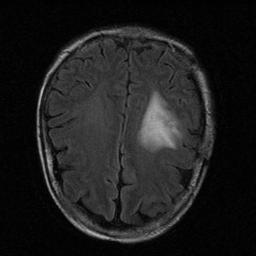
\includegraphics[width=0.95\textwidth]{images/IRMcoupe17-t2.jpg}
	\caption{IRM après traitement}\label{irm2}
    \end{subfigure}
\end{figure}

Nous utiliserons trois techniques pour segmenter la tumeur:
\begin{itemize}
	\item la binarisation par seuillage
	\item l'algorithme des fuzzy c-means
	\item les champs de Markov
\end{itemize}

\bigskip

Nous comparerons les résultats obtenus avec chacun de ces algorithmes afin de comparer leur efficacité et leur stabilité.